\chapter*{Explicación del Gráfico}
\addcontentsline{toc}{chapter}{Explicación del Gráfico}
Debido a que diferentes muestras de madera para la tapa armónica deben recibir tratamientos distintos en cuanto a la graduación, no se proporcionan valores para los espesores; pero, en lugar de cifras, se emplea el sombreado como medio para indicar valores cuantitativos relativos. El único experimento mencionado en el texto, y que tiene en vista la máxima uniformidad de la potencia del tono, operó para aumentar los tonos altísimos en un grado más marcado que los tonos de tono más bajo. Debido a que la potencia en los tonos altísimos es deseable y difícil de asegurar, este método de graduación se registra, con la esperanza de que futuros estudiantes del violín puedan continuar el experimento de acortar la longitud de la actividad de la tapa armónica para aumentar el volumen de los tono más alto. La prueba indudablemente determinará una mejor proporción que 2/3 para acortar la actividad de la fibra debajo de las cuerdas más ligeras.


\begin{center}
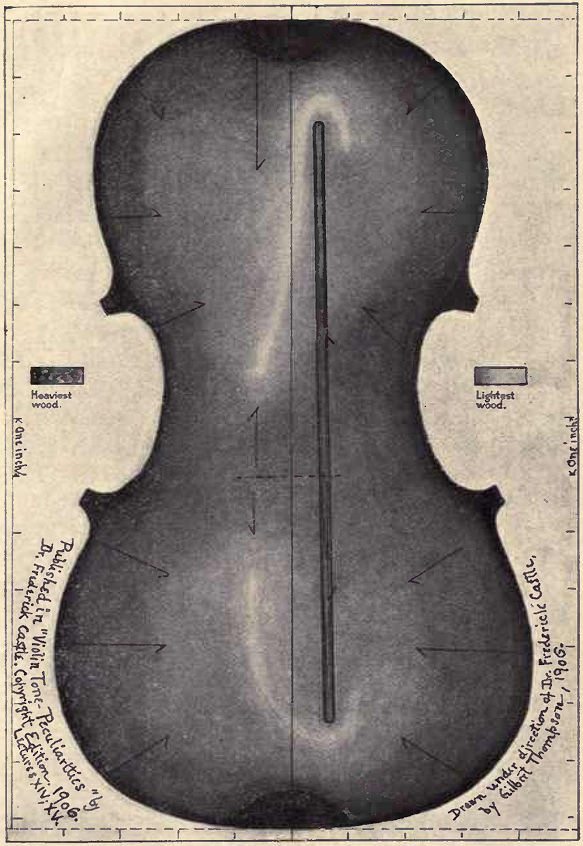
\includegraphics[width=1\textwidth]{../img/grafico.png} % Reemplaza "grafico.jpg" con el nombre del archivo de la imagen
\end{center}
